\section{The polar coefficients at the cusp $\infty$}\label{sec:polarinf}

\begin{theorem}\label{thm:Pinf}
Let $m\ge1$, $\nu\in\frac12\ZZ$ and $0\le\tilde\ell<2m$ with $4m\nu-\tilde\ell^2<0$. Then
\[
c^F_m(2\nu,\tilde\ell)=a_I(\nu,\tilde\ell),
\]
with $a_I$ the wall sum \eqref{eq:Pinf}. Consequently (P$\infty$) of Section~\ref{sec:rademacher} holds: the principal part of $\varphi^F_m$ at the cusp $\infty$ in the frame $I$ is given by \eqref{eq:Pinf}, and in the frame $T$, which is obtained by $\sigma\mapsto\sigma+1$, that is $x\mapsto-x$, by $a_T=(-1)^{2\nu}a_I$.
\end{theorem}

In outline: the product converges on a tube domain and defines a meromorphic function whose poles lie over walls in the space of imaginary parts; the walls are the Farey geodesics with an even denominator; across each wall the Fourier coefficients of $1/\Phit_6$ jump by a product of two coefficients $d_1$ (a residue computation, transported by $\Gamma_0(2)$); the polar coefficients of $\varphi^F_m$ are the coefficients in one chamber $K_0$; and following a vertical path from $K_0$ to a chamber in which the coefficient vanishes gives the wall sum. Every statement below is proved here; from Section~\ref{sec:setup} we take the definitions \eqref{eq:genera}, \eqref{eq:product}, \eqref{eq:polar}, the identities \eqref{eq:phim1}, \eqref{eq:Ll} (rearrangements of the product formula) and Lemma~\ref{lem:modular}, and from Section~\ref{sec:reduction} Lemma~\ref{lem:fricke}.

\subsection{Notation}
Write $\Omega=\begin{psmallmatrix}\rho&v\\v&\sigma\end{psmallmatrix}$, $\Omega=X+iY$ with
\[
Y=\begin{pmatrix}M_1&M_3\\M_3&M_2\end{pmatrix}=\operatorname{Im}\Omega,
\]
and let $\mathcal P$ be the open cone of positive definite real symmetric $2\times2$ matrices. A \emph{charge} is a triple $T=(m,\nu,\ell)\in\Lambda:=\ZZ\times\frac12\ZZ\times\ZZ$; it stands for the monomial $\e(\langle T,\Omega\rangle)$ with
\[
\langle T,\Omega\rangle=m\rho+\nu\sigma+\ell v=\operatorname{tr}(S_T\Omega),\qquad S_T=\begin{pmatrix}m&\ell/2\\\ell/2&\nu\end{pmatrix},\qquad N(T):=4\det S_T=4m\nu-\ell^2 ,
\]
so that $\e(\langle T,\Omega\rangle)=\e(m\rho)x^{2\nu}y^\ell$. In the notation of Lemma~\ref{lem:fricke}, the factor $1-x^A\e(B\rho)y^j$ of \eqref{eq:product} is $1-\e(\langle g,\Omega\rangle)$ with the \emph{factor charge} $g=(B,A/2,j)$, its exponent is $E(g):=E(A,B,j)$, and $N(g)=2AB-j^2$. Let
\[
\mathcal I=\{(B,A/2,j):\ A,B\in\ZZ_{\ge0},\ j\in\ZZ,\ j<0\text{ if }A=B=0\},\qquad \varrho=(1,\tfrac12,1),
\]
so that \eqref{eq:product} reads $\Phit_6=\e(\langle\varrho,\Omega\rangle)\prod_{g\in\mathcal I}\big(1-\e(\langle g,\Omega\rangle)\big)^{E(g)}$.

The coefficient $c^{(r,s)}_b(N)$ of \eqref{eq:product} is the coefficient of $q^n\zeta^j$ in $F^{(r,s)}$ for any $(n,j)$ with $4n-j^2=N$, $j\equiv b\pmod 2$: this is the usual consequence of the elliptic invariance of index one under $z\mapsto z+\lambda\tau+\mu$, $\lambda,\mu\in\ZZ$. Since the expansions of the $F^{(r,s)}$ contain no negative powers of $q$, taking $j=b\in\{0,1\}$ gives
\begin{equation}\label{eq:cvanish}
c^{(r,s)}_b(N)=0\quad\text{for }N<-1,\qquad\text{hence}\qquad E(g)=0\quad\text{if }N(g)<-1.
\end{equation}

For $Y\in\mathcal P$ put
\[
\tau_Y=\frac{-M_3+i\sqrt{\det Y}}{M_2}\in\mathbb H,\qquad\text{so that}\qquad Y=\frac{\sqrt{\det Y}}{\operatorname{Im}\tau_Y}\begin{pmatrix}|\tau_Y|^2&-\operatorname{Re}\tau_Y\\-\operatorname{Re}\tau_Y&1\end{pmatrix}.
\]
The map $Y\mapsto(\tau_Y,\det Y)$ is a bijection $\mathcal P\to\mathbb H\times\mathbb R_{>0}$, and for $\tau=\tau_Y=\mathsf x+i\mathsf y$,
\begin{equation}\label{eq:pairing}
\langle T,Y\rangle=\frac{\sqrt{\det Y}}{\mathsf y}\big(m|\tau|^2-\ell\,\mathsf x+\nu\big).
\end{equation}
For $A=\begin{psmallmatrix}a&b\\c&d\end{psmallmatrix}\in SL_2(\ZZ)$ the substitution $\Omega\mapsto A\Omega A^T$ preserves $\det Y$, and
\begin{equation}\label{eq:tauaction}
\tau_{AYA^T}=M_A\,\tau_Y,\qquad M_A=\begin{pmatrix}a&-b\\-c&d\end{pmatrix}.
\end{equation}
Indeed $Y=\frac{\sqrt{\det Y}}{\mathsf y}\operatorname{Re}(zz^*)$ with $z=(-\tau,1)^T$, and $Az=(-c\tau+d)\,(-\tau',1)^T$ with $\tau'=M_A\tau$, $\operatorname{Im}\tau'=\mathsf y/|{-c\tau+d}|^2$. Since $A\mapsto M_A$ is conjugation by $\operatorname{diag}(1,-1)$, it maps $\Gamma_0(2)$ onto itself. On charges, $\langle T,A\Omega A^T\rangle=\langle A^{\ast}T,\Omega\rangle$ with $S_{A^\ast T}=A^TS_TA$, that is
\begin{equation}\label{eq:chargeaction}
A^\ast(m,\nu,\ell)=\big(ma^2+\ell ac+\nu c^2,\ mb^2+\ell bd+\nu d^2,\ 2mab+\ell(ad+bc)+2\nu cd\big),
\end{equation}
which maps $\Lambda$ to itself when $c$ is even.

\subsection{Convergence}

\begin{lemma}\label{lem:growth}
There are constants $K,\kappa>0$ with $|c^{(r,s)}_b(N)|\le Ke^{\kappa\sqrt{N+1}}$ for all $r,s,b$ and $N\ge-1$.
\end{lemma}

\begin{proof}
For a series $f=\sum a(n,j)q^n\zeta^j$ with $n\in\frac14\ZZ$ write $f^+=\sum_n\big(\sum_j|a(n,j)|\big)q^n$; then $(fg)^+\le f^+g^+$ coefficientwise. By \eqref{eq:genera} each $F^{(r,s)}$ is a linear combination of $\theta_k(\tau,z)^2/\theta_k(\tau)^2$ ($k=2,3,4$), of $\theta_1(\tau,z)^2/\eta(\tau)^6$ and of its products with $\fE(\tau)$, $\fE(\tau/2)$, $\fE((\tau+1)/2)$. The coefficients of $\theta_k(\tau,z)^2q^{-\epsilon_k}$ ($\epsilon_1=\epsilon_2=\frac14$, $\epsilon_3=\epsilon_4=0$) in $q^{1/2}$ are bounded by the number of representations of an integer as a sum of two squares, hence by a polynomial; those of $\fE$ are $24\sigma_1^{\rm odd}(n)\le24n^2$. The remaining factors $q^{\epsilon_k}/\theta_k(\tau)^2$ and $q^{1/4}/\eta(\tau)^6$ are eta quotients, $\theta_2=2\eta(2\tau)^2/\eta(\tau)$, $\theta_3=\eta(\tau)^5/(\eta(\tau/2)^2\eta(2\tau)^2)$, $\theta_4=\eta(\tau/2)^2/\eta(\tau)$, so their coefficients in $X=q^{1/2}$ are bounded in absolute value by those of $\prod_{i\ge1}(1-X^i)^{-E_0}$ for a fixed $E_0$. Let $p_E(k)$ be the coefficient of $X^k$ in $\prod_i(1-X^i)^{-E}$. For $0<X<1$, $-\log(1-X^i)=\sum_{n\ge1}X^{in}/n$ and $X^n/(1-X^n)\le X/(n(1-X))$ give $\log\prod_i(1-X^i)^{-1}\le\pi^2/(6(1-X))$, hence $p_E(k)\le X^{-k}\exp(E\pi^2/(6(1-X)))$. With $X=1-(k+1)^{-1/2}$ and $-\log(1-u)\le2u$ for $u\le\frac12$ this gives $p_E(k)\le\exp\big((2+E\pi^2/6)\sqrt{k+1}\big)$ for $k\ge3$. Multiplying the finitely many majorants, the coefficient of $q^n$ in $F^{(r,s)+}$ is at most $K_1(n+1)^{B_1}e^{\kappa_1\sqrt{2n+1}}$. Finally $c^{(r,s)}_b(N)$ is the coefficient of $q^n\zeta^b$ with $n=(N+b^2)/4\le(N+1)/4$.
\end{proof}

Fix $K,\kappa$ as in Lemma~\ref{lem:growth}, put $R_0=(\kappa/\pi)^2$ and
\[
\mathcal D=\{Y\in\mathcal P:\ \det Y>R_0\},\qquad \mathcal T=\{\Omega:\ \operatorname{Im}\Omega\in\mathcal D\}.
\]
The set $\mathcal D$ is connected (it is $\mathbb H\times(R_0,\infty)$ under $Y\mapsto(\tau_Y,\det Y)$), and so is $\mathcal T$.

\begin{lemma}\label{lem:Nm1}
Let $g=(B,k',j)\in\mathcal I$ with $N(g)=-1$. Then $E(g)=2$ if $k'\in\ZZ$ and $B$ is even, and $E(g)=0$ otherwise. If $N(g)\ge0$, then $S_g$ is positive semidefinite and nonzero.
\end{lemma}

\begin{proof}
Let $N=-1$, so $j$ is odd. The coefficient $c^{(r,s)}_1(-1)$ is the coefficient of $q^0\zeta$ in $F^{(r,s)}$. By \eqref{eq:genera}, with $\pB=\zeta+10+\zeta^{-1}+O(q)$, $\pA=\zeta-2+\zeta^{-1}+O(q)$ and $\fE=1+O(q)$, it equals $1,1,0,0$ for $(r,s)=(0,0),(0,1),(1,0),(1,1)$. Hence $E(g)=1+(-1)^B$ if $r=0$, that is $k'\in\ZZ$, and $E(g)=0$ if $r=1$. If $N(g)\ge0$ then $B,k'\ge0$ and $4Bk'\ge j^2$, so $S_g$ is positive semidefinite; it is zero only for $g=(0,0,0)\notin\mathcal I$.
\end{proof}

A factor charge $g\in\mathcal I$ with $N(g)=-1$ and $E(g)\ne0$ is called a \emph{wall charge}, and $\{Y:\langle g,Y\rangle=0\}$ its \emph{wall}. By \eqref{eq:pairing} the wall of $g=(B,k',j)$ is the cone over the geodesic
\begin{equation}\label{eq:geodesic}
B|\tau|^2-j\,\mathsf x+k'=0
\end{equation}
in $\mathbb H$, whose endpoints are the roots of $Bt^2-jt+k'$, a polynomial of discriminant $j^2-4Bk'=1$. A \emph{Farey edge} is a pair of fractions $a/c,b/d\in\mathbb Q\cup\{\infty\}$ in lowest terms, $c,d\ge0$, $\infty=1/0$, with $|ad-bc|=1$, viewed as the geodesic of $\mathbb H$ joining them; it is \emph{even} if $cd$ is even and \emph{odd} if $c,d$ are both odd. Two adjacent fractions cannot both have even denominators, so every Farey edge is either even or odd.

\begin{lemma}\label{lem:wallsfarey}
The map $g\mapsto$\eqref{eq:geodesic} is a bijection from the set of wall charges onto the set of even Farey edges. If the edge of $g$ joins $a/c$ and $b/d$ with $c,d\ge1$, then $g=(cd,ab,ad+bc)$ and
\begin{equation}\label{eq:wallpair}
\langle g,Y\rangle=\frac{\sqrt{\det Y}}{\mathsf y}\,Q,\qquad Q=\operatorname{Re}\big[(c\tau-a)(d\bar\tau-b)\big],\qquad Q^2+\mathsf y^2=|c\tau-a|^2\,|d\tau-b|^2,
\end{equation}
with $\tau=\tau_Y$; $\langle g,Y\rangle>0$ outside the half-disc bounded by the edge. The vertical edges $\{\infty,n\}$, $n\in\ZZ$, are the walls of $(0,n,1)$ for $n\ge1$ and $(0,-n,-1)$ for $n\le0$, with $\langle g,Y\rangle>0$ on the side $\mathsf x<n$, respectively $\mathsf x>n$.
\end{lemma}

\begin{proof}
Let $g=(B,k',j)$ be a wall charge, so $k'\in\ZZ$ and $B$ is even, and $\gcd(B,j,k')=1$ because its square divides the discriminant $1$. If $B>0$, the roots $(j\pm1)/2B$ are rational, so by Gauss's lemma $Bt^2-jt+k'=(ct-a)(dt-b)$ with integers, and comparing coefficients $cd=B$, $ad+bc=j$, $ab=k'$ and $(ad-bc)^2=j^2-4Bk'=1$. Since $cd=B>0$ we may take $c,d\ge1$; then $cd=B$ is even. If $B=0$ then $j=\pm1$ and the root is $k'/j=jk'$; the conditions $k'\ge0$, and $j<0$ if $k'=0$, give each integer exactly once, as stated. Conversely, for an even edge $\{a/c,b/d\}$ with $c,d\ge1$ the charge $\pm(cd,ab,ad+bc)$ with the sign making $cd>0$ has $N=4abcd-(ad+bc)^2=-(ad-bc)^2=-1$, $k'=ab\in\ZZ$ and $B=cd$ even, so $E=2$ by Lemma~\ref{lem:Nm1}; it lies in $\mathcal I$ because $ab\ge0$: the two endpoints lie on the same side of $0$, since by Lemma~\ref{lem:farey}(F1) below a Farey edge does not cross the edge $\{0,\infty\}$. For \eqref{eq:wallpair}, $(c\tau-a)(d\bar\tau-b)=cd|\tau|^2-(ad\bar\tau+bc\tau)+ab$ has real part $B|\tau|^2-j\mathsf x+k'$ and imaginary part $(ad-bc)\mathsf y=\pm\mathsf y$; combine with \eqref{eq:pairing}. The sign statements follow from \eqref{eq:geodesic}.
\end{proof}

\begin{lemma}\label{lem:farey}
\begin{enumerate}
\item[(F3)] If $a/c<e/f<b/d$ with $bc-ad=1$, $c,d,f\ge1$, then $f\ge c+d$.
\item[(F1)] Two distinct Farey edges do not cross: their intersection in $\mathbb H$ is empty.
\item[(F0)] For every compact set $\mathcal K\subset\mathbb H$ only finitely many Farey edges meet $\mathcal K$; more precisely an edge with $c,d\ge1$ meeting $\{\operatorname{Im}\tau\ge\mathsf y_0\}$ has $cd\le1/(2\mathsf y_0)$.
\end{enumerate}
\end{lemma}

\begin{proof}
(F3) $e/f-a/c\ge1/(cf)$ and $b/d-e/f\ge1/(df)$, and their sum is $1/(cd)$, so $1/(cd)\ge(c+d)/(cdf)$. (F1) Two geodesics cross only if their endpoints interleave. A vertical edge $\{\infty,n\}$ would have $n$ strictly inside an edge $(a/c,b/d)$ with $c,d\ge1$, so $1\ge c+d$ by (F3), which is impossible. For two edges $(a/c,b/d)$, $(a'/c',b'/d')$ with all denominators $\ge1$ and interleaving endpoints, one endpoint of each lies strictly inside the other; by (F3) its denominator is at least the sum of the denominators of the other edge, and the two inequalities contradict each other. (F0) The edge is a semicircle of radius $1/(2cd)$, and its centre lies within $1$ of $\operatorname{Re}\tau$; vertical edges meet $\mathcal K$ only for finitely many $n$.
\end{proof}

\begin{proposition}\label{prop:convergence}
\begin{enumerate}
\item[(i)] For every compact $\mathcal K\subset\mathcal D$ and every $X_0$ the set of wall charges with $\langle g,Y\rangle\le X_0$ for some $Y\in\mathcal K$ is finite, and $\sum_{g\in\mathcal I}|E(g)|\,e^{-2\pi\langle g,Y\rangle}$, taken over the $g$ with $\langle g,Y\rangle>0$, converges uniformly on $\mathcal K$.
\item[(ii)] The product \eqref{eq:product} converges absolutely and locally uniformly on $\mathcal T$, and $\Phit_6$ is holomorphic on $\mathcal T$.
\item[(iii)] The zeros of $\Phit_6$ in $\mathcal T$ are the points with $\langle g,\Omega\rangle\in\ZZ$ for a wall charge $g$; there $\operatorname{Im}\Omega$ lies on the wall of $g$, and the zero is a double zero of the factor $(1-\e(\langle g,\Omega\rangle))^2$, all other factors being nonzero. Hence $\mathcal F:=1/\Phit_6$ is meromorphic on $\mathcal T$ and holomorphic on the tube over the complement of the walls.
\end{enumerate}
\end{proposition}

\begin{proof}
(i) Factors with $N(g)<-1$ have $E(g)=0$ by \eqref{eq:cvanish}. For $N(g)\ge0$, $S_g$ is positive semidefinite (Lemma~\ref{lem:Nm1}), and for positive semidefinite $S$ and $Y\in\mathcal P$, $\operatorname{tr}(SY)\ge2\sqrt{\det S\det Y}$ and $\operatorname{tr}(SY)\ge\lambda_{\min}(Y)\operatorname{tr}S$. Hence
\[
2\pi\langle g,Y\rangle\ge\pi\sqrt{N(g)\det Y}+\pi\lambda_{\min}(Y)(B+k').
\]
By Lemma~\ref{lem:growth} and $\pi\sqrt{\det Y}\ge\kappa$ on $\mathcal D$, $|E(g)|e^{-2\pi\langle g,Y\rangle}\le4Ke^{\kappa}e^{-\pi\lambda_{\min}(Y)(B+k')}$, and for given $(B,k')$ there are at most $4(B+k')+1$ values of $j$. Since $\lambda_{\min}$ is continuous and positive, these terms are summable uniformly on $\mathcal K$. For a non-vertical wall charge, $Q=cd\big(|\tau-\omega|^2-(2cd)^{-2}\big)\ge-1/(4cd)$, $\omega$ the centre of the edge, so by \eqref{eq:wallpair} and $|c\tau-a|\ge c\mathsf y$, $|d\tau-b|\ge d\mathsf y$, the inequality $\langle g,Y\rangle\le X$ implies $cd\,\mathsf y^2\le Z$ and $|c\mathsf x-a|\le Z/(d\mathsf y)$ with $Z=\big(\max(X\mathsf y/\sqrt{\det Y},\frac14)^2+\mathsf y^2\big)^{1/2}$; on $\mathcal K$ the quantities $\mathsf x,\mathsf y,\det Y$ are bounded and $\mathsf y,\det Y$ bounded below, so the number of wall charges with $\langle g,Y\rangle\le X$ is $O((1+X)^3)$ uniformly on $\mathcal K$ (vertical walls contribute $O(1+X)$). This gives finiteness and uniform convergence of the sum over wall charges.
(ii) By (i), on a neighbourhood of a compact set only finitely many factors have $\langle g,Y\rangle\le\frac{1}{2\pi}\log2$, and the remaining ones satisfy $|\e(\langle g,\Omega\rangle)|\le\frac12$ with $\sum|E(g)||\e(\langle g,\Omega\rangle)|$ uniformly convergent; their product converges absolutely and uniformly to a holomorphic function without zeros, and the finitely many others are entire. (iii) The infinite part has no zeros. Among the finitely many remaining factors, those with $N(g)\ge0$ satisfy $|\e(\langle g,\Omega\rangle)|<1$, so only wall charges can vanish, exactly when $\langle g,\Omega\rangle\in\ZZ$, which forces $\langle g,Y\rangle=0$. Distinct Farey edges are disjoint in $\mathbb H$ (Lemma~\ref{lem:farey}(F1)), so at such a point no other factor vanishes.
\end{proof}

\subsection{Chambers and Fourier coefficients}
The \emph{walls} in $\mathbb H$ are the even Farey edges; by (F0) their union is closed. A \emph{chamber} is a connected component $C$ of the complement of the walls in $\mathbb H$, and we put $\tilde C=\{Y\in\mathcal D:\tau_Y\in C\}$, which is connected. Let $K_0$ be the open ideal quadrilateral with vertices $0,\frac12,1,\infty$, and $K_0'$ the one with vertices $-1,-\frac12,0,\infty$.

\begin{lemma}\label{lem:chamberexp}
Let $C$ be a chamber.
\begin{enumerate}
\item[(i)] For each wall charge $g$ the sign of $\langle g,Y\rangle$ is constant on $\tilde C$, and the set $\mathcal I^-_C$ of wall charges with $\langle g,Y\rangle<0$ on $\tilde C$ is finite.
\item[(ii)] On the tube over $\tilde C$,
\[
\mathcal F(\Omega)=\e\Big(-\Big\langle\varrho+2\sum_{g\in\mathcal I^-_C}g,\ \Omega\Big\rangle\Big)\prod_{g\in\mathcal I_C}\big(1-\e(\langle g,\Omega\rangle)\big)^{-E(g)},\qquad \mathcal I_C=(\mathcal I\setminus\mathcal I^-_C)\cup(-\mathcal I^-_C),
\]
with $E(-g):=E(g)$, and $\langle g,Y\rangle>0$ for every $g\in\mathcal I_C$ with $E(g)\ne0$ and $Y\in\tilde C$.
\item[(iii)] Expanding each factor binomially gives $\mathcal F(\Omega)=\sum_{T\in\Lambda}d(T;C)\,\e(\langle T,\Omega\rangle)$ with integers $d(T;C)$, absolutely and locally uniformly convergent on the tube over $\tilde C$, and for every $Y\in\tilde C$
\begin{equation}\label{eq:dintegral}
d(T;C)=\frac12\int_0^1\!\!\int_0^2\!\!\int_0^1\mathcal F(X+iY)\,\e(-\langle T,X+iY\rangle)\,dX_v\,dX_\sigma\,dX_\rho .
\end{equation}
\end{enumerate}
\end{lemma}

\begin{proof}
(i) $\langle g,Y\rangle$ vanishes only on the wall of $g$, which does not meet $C$; the finiteness is Proposition~\ref{prop:convergence}(i) at one point. (ii) Use $(1-\e(w))^{-2}=\e(-2w)(1-\e(-w))^{-2}$ for $g\in\mathcal I^-_C$, and Lemma~\ref{lem:Nm1} for $N(g)\ge0$. (iii) Each factor $(1-u)^{-E}=\sum_k\binom{-E}{k}(-u)^k$ is majorised by $(1-|u|)^{-|E|}$, and $\prod(1-|u_g|)^{-|E(g)|}$ converges locally uniformly by Proposition~\ref{prop:convergence}(i). For given $T$ only finitely many products of monomials contribute, because $\{g\in\mathcal I_C:\,0<\langle g,Y\rangle\le X_0\}$ is finite for every $X_0$ (Proposition~\ref{prop:convergence}(i) for the walls, and $\lambda_{\min}(Y)(B+k')\le\langle g,Y\rangle$ for $N(g)\ge0$); so $d(T;C)$ is a finite sum of integers. $\mathcal F$ has period $1$ in $\rho$ and $v$ and period $2$ in $\sigma$, and \eqref{eq:dintegral} follows from absolute convergence.
\end{proof}

The edge $(0,1)$ is odd, so $K_0$ is the set of $\tau$ with $0<\mathsf x<1$ lying outside the half-discs on $(0,\frac12)$ and $(\frac12,1)$. Every wall charge is positive on $\tilde K_0$. For the vertical walls this is Lemma~\ref{lem:wallsfarey}. By (F3) no Farey edge with $c,d\ge1$ contains $0$ or $1$ strictly inside its interval, and only $(0,1)$ contains $\frac12$; so the half-disc of a non-vertical wall lies in $\{\mathsf x\le0\}$, in $\{\mathsf x\ge1\}$, or in the closed half-disc on $(0,\frac12)$ or on $(\frac12,1)$, and every point of $K_0$ is outside it. Hence $\mathcal I^-_{K_0}=\varnothing$, the expansion of Lemma~\ref{lem:chamberexp} on $\tilde K_0$ is the expansion of the product \eqref{eq:product} itself, and $K_0$ is a chamber: it is open, connected, contains no wall point, and its boundary consists of wall points.

\subsection{Symmetries}

\begin{lemma}\label{lem:symmetries}
For $\Omega\in\mathcal T$:
\begin{enumerate}
\item[(i)] $\Phit_6(E\Omega E^T)=\Phit_6(\Omega)$ for $E=\begin{psmallmatrix}1&1\\0&1\end{psmallmatrix}$, that is $\Phit_6(\rho+2v+\sigma,\sigma,v+\sigma)=\Phit_6(\rho,\sigma,v)$;
\item[(ii)] $\Phit_6(\rho,\sigma,-v)=\Phit_6(\rho,\sigma,v)$;
\item[(iii)] $\Phit_6(\sigma/2,2\rho,v)=\Phit_6(\rho,\sigma,v)$;
\item[(iv)] $\Phit_6(A\Omega A^T)=\Phit_6(\Omega)$ for every $A\in\Gamma_0(2)$, and consequently $d(T;C')=d(A^\ast T;C)$ whenever $C'=M_A(C)$.
\end{enumerate}
\end{lemma}

\begin{proof}
All substitutions preserve $\mathcal D$ (they act on $Y$ by $Y\mapsto PYP^T$ with $\det P=\pm1$), so both sides are absolutely convergent products on $\mathcal T$ and may be compared factor by factor.

(i) $\langle g,E\Omega E^T\rangle=\langle E^\ast g,\Omega\rangle$ with $E^\ast(B,k',j)=(B,k'+B+j,j+2B)$ by \eqref{eq:chargeaction}. This map preserves $N$, $B$, $j\bmod2$ and $2k'\bmod2$, hence $E(E^\ast g)=E(g)$. Among the charges with $N\ge-1$ it maps $\mathcal I$ onto $(\mathcal I\setminus\{(0,1,1)\})\cup\{(0,-1,-1)\}$: for $B>0$, $4B(k'+B+j)=N+(j+2B)^2\ge0$ (if $j+2B=0$ then $N\equiv0\pmod 4$, so $N\ge0$), and the same holds for $E^{-1}$; for $B=0$ only $j\in\{0,\pm1\}$ occur, $(0,k',0)$ is fixed, $(0,k',1)\mapsto(0,k'+1,1)$ and $(0,k',-1)\mapsto(0,k'-1,-1)$. Both exceptional charges have $E=2$, so the product over $\mathcal I$ acquires the factor $(1-\e(-\sigma-v))^2/(1-\e(\sigma+v))^2=\e(-2\sigma-2v)$, while $\langle\varrho,E\Omega E^T\rangle=\langle\varrho,\Omega\rangle+2\sigma+2v$.

(ii) $v\mapsto-v$ maps $(B,k',j)$ to $(B,k',-j)$, which preserves $E$ and maps $\mathcal I$ onto itself except that $(0,0,-1)$ becomes $(0,0,1)$; the factors with $E\ne0$ and $A=B=0$ have $j=-1$ by \eqref{eq:cvanish}. Since $\e(v)(1-\e(-v))^2=\e(-v)(1-\e(v))^2$, the two products agree.

(iii) is Lemma~\ref{lem:fricke}: the factor sets correspond under $(A,B,j)\mapsto(B,A,j)$ with equal exponents, and the products converge absolutely on $\mathcal T$.

(iv) Let $V(\Omega)=W\Omega W^T$ with $W=\begin{psmallmatrix}0&-1/\sqrt2\\\sqrt2&0\end{psmallmatrix}$, so $V(\rho,\sigma,v)=(\sigma/2,2\rho,-v)$ and $\Phit_6\circ V=\Phit_6$ by (ii) and (iii). Since $WEW^{-1}=\begin{psmallmatrix}1&0\\-2&1\end{psmallmatrix}=:L^{-1}$, (i) and $V$-invariance give $\Phit_6(L^{-1}\Omega L^{-T})=\Phit_6(E(W^{-1}\Omega W^{-T})E^T)=\Phit_6(W^{-1}\Omega W^{-T})=\Phit_6(\Omega)$. The matrices $E$, $L$ and $-I$ generate $\Gamma_0(2)$: for $A=\begin{psmallmatrix}a&b\\c&d\end{psmallmatrix}\in\Gamma_0(2)$ with $c\ne0$, $a$ is odd; replacing $A$ by $E^kA$ makes $|a|\le|c|/2$, and then for suitable $k$ the matrix $L^kA\in\Gamma_0(2)$ has lower left entry $c+2ka$ with $|c+2ka|\le|a|<|c|$; after finitely many steps $c=0$ and $A=\pm E^k$. Finally, if $C'=M_A(C)$ and $Y\in\tilde C'$, then $A^{-1}YA^{-T}\in\tilde C$ by \eqref{eq:tauaction}, and
\[
\mathcal F(\Omega)=\mathcal F(A^{-1}\Omega A^{-T})=\sum_{S}d(S;C)\,\e(\langle S,A^{-1}\Omega A^{-T}\rangle),
\]
so the coefficient of $\e(\langle T,\Omega\rangle)$ is $d(S;C)$ with $(A^{-1})^\ast S=T$, that is $S=A^\ast T$.
\end{proof}

\subsection{The chambers}
For an even or odd Farey edge $e=(a/c,b/d)$ with $c,d\ge1$ let $\Delta(e)$ be the open ideal triangle with vertices $a/c$, $b/d$ and the mediant $(a+b)/(c+d)$, that is, the set of points inside the half-disc of $e$ and outside the half-discs of its two \emph{children} $(a/c,(a+b)/(c+d))$ and $((a+b)/(c+d),b/d)$; for $n\in\ZZ$ let $\Delta(n)$ be the open triangle with vertices $n,n+1,\infty$.

\begin{lemma}\label{lem:tess}
\begin{enumerate}
\item[(i)] The triangles $\Delta(e)$, $\Delta(n)$ are pairwise disjoint, and $\mathbb H$ is the union of their closures.
\item[(ii)] Each triangle has exactly one odd side.
\item[(iii)] The chambers are exactly the ideal quadrilaterals $Q(e_0)=\Delta\cup\Delta'\cup e_0$, where $e_0$ is an odd edge and $\Delta,\Delta'$ are the two triangles having $e_0$ as a side. In particular $K_0=Q((0,1))$ and $K_0'=Q((-1,0))$.
\item[(iv)] $\Gamma_0(2)$ acts transitively on the odd edges; hence every chamber is $M(K_0)$ for some $M\in\Gamma_0(2)$, and every chamber is $M_A(K_0)$ for some $A\in\Gamma_0(2)$.
\end{enumerate}
\end{lemma}

\begin{proof}
(i) Let $\tau$ lie on no Farey edge. By (F0) only finitely many edges have $\tau$ in their half-disc, and by (F1) their intervals are nested. If there is none, $n<\operatorname{Re}\tau<n+1$ for some $n$, and $\tau$ is not in the half-disc of $(n,n+1)$, so $\tau\in\Delta(n)$. Otherwise let $e$ be the innermost one; $\tau$ is not in the half-disc of a child of $e$, which would be a smaller such edge, so $\tau\in\Delta(e)$. Points on edges lie in the closure of adjacent triangles by the same argument applied to nearby points. Moreover no edge meets an open triangle: by (F1) and the argument below, an edge meeting the half-disc of $e$ is $e$, a child of $e$, or lies under a child. Hence the open triangles are the components of the complement of all Farey edges. For disjointness, suppose $\tau\in\Delta(e)\cap\Delta(e')$ with $e\ne e'$; then $\tau$ is in both half-discs, so one interval, say that of $e'$, lies strictly inside that of $e=(a/c,b/d)$ and has an endpoint strictly between $a/c$ and $b/d$. That endpoint has denominator at least $c+d$ by (F3); if the interval of $e'$ contained the mediant strictly inside, (F3) applied to $e'$ would bound the sum of its denominators by $c+d$, which is impossible. So $e'$ lies in the closed half-disc of a child of $e$, and $\tau$ lies inside that child's half-disc, a contradiction. The cases involving $\Delta(n)$ are similar and easier.
(ii) The vertices of $\Delta(e)$ have denominators $c,d,c+d$, and those of $\Delta(n)$ have $1,1,0$; exactly one is even, since no two adjacent fractions both have even denominators. The side joining the two odd ones is odd, the other two are even.
(iii) By (i), (F0) and (F1), every edge is a side of exactly two triangles, one on each side: near an interior point of the edge, each side is covered by the closure of a single triangle. By (ii) the sets $Q(e_0)$ are pairwise disjoint; each is open and connected and contains no wall point, and their union is the complement of the walls. So they are the components. The triangles $\Delta(0)$ and $\Delta((0,1))$ share the odd edge $(0,1)$, which gives $K_0$, and similarly for $K_0'$.
(iv) A matrix of $SL_2(\ZZ)$ maps Farey edges to Farey edges and, if it lies in $\Gamma_0(2)$, preserves the parity of denominators: $\begin{psmallmatrix}\alpha&\beta\\\gamma&\delta\end{psmallmatrix}(a/c)$ has denominator $\gamma a+\delta c\equiv c\pmod2$. So $\Gamma_0(2)$ permutes triangles, walls, odd edges and chambers, and maps $Q(e_0)$ to $Q(Me_0)$. Given an odd edge $(u_1/v_1,u_2/v_2)$ with $u_1v_2-u_2v_1=1$, the matrix $M=\begin{psmallmatrix}u_1-u_2&u_2\\v_1-v_2&v_2\end{psmallmatrix}$ lies in $\Gamma_0(2)$ and maps $1\mapsto u_1/v_1$, $0\mapsto u_2/v_2$. The last statement follows from \eqref{eq:tauaction}, since $A\mapsto M_A$ is a bijection of $\Gamma_0(2)$.
\end{proof}

\subsection{The jump across a wall}

\begin{lemma}[Jump lemma]\label{lem:jump}
For every charge $T=(m,\nu,\ell)$,
\[
d(T;K_0)-d(T;K_0')=-\ell\,d_1(m)\,d_1(2\nu).
\]
\end{lemma}

\begin{proof}
The wall between $K_0$ and $K_0'$ is $W_0=\{\operatorname{Re}\tau=0\}=\{M_3=0\}$, the wall of $g_0=(0,0,-1)$, with $\langle g_0,Y\rangle=-M_3>0$ on $\tilde K_0$. Fix $Y_0=(M_1,M_2,0)\in\mathcal D$ and a compact neighbourhood $U$ of $Y_0$ in $\mathcal D$, symmetric under $M_3\mapsto-M_3$, which meets no wall other than $W_0$ (Lemma~\ref{lem:farey}(F0),(F1)) and whose two halves $U\cap\{M_3<0\}$, $U\cap\{M_3>0\}$ lie in $\tilde K_0$, $\tilde K_0'$. On the tube over $U$ all factor charges $g\ne g_0$ with $E(g)\ne0$ have $\langle g,Y\rangle>0$, and since
\[
\e(-v)\big(1-\e(-v)\big)^{-2}=-\frac1{4\sin^2\pi v},
\]
we have $\mathcal F=-H/(4\sin^2\pi v)$ with
\[
H(\Omega)=\e\big(-\rho-\tfrac\sigma2\big)\prod_{g\in\mathcal I,\ g\ne g_0}\big(1-\e(\langle g,\Omega\rangle)\big)^{-E(g)},
\]
holomorphic on the tube over $U$. By Lemma~\ref{lem:symmetries}(ii) $\mathcal F$ is even in $v$, hence so is $H$.

Take $Y_\pm=(M_1,M_2,\mp\epsilon)\in U$, so $Y_+\in\tilde K_0$, $Y_-\in\tilde K_0'$, and apply \eqref{eq:dintegral}. For fixed real parts of $\rho,\sigma$ the function $v\mapsto\mathcal F e(-\langle T,\Omega\rangle)$ is $1$-periodic and meromorphic on $|\operatorname{Im}v|\le\epsilon$ with poles only at $v\in\ZZ$. The difference of the integrals over $\operatorname{Im}v=-\epsilon$ and $\operatorname{Im}v=\epsilon$ is the integral over the positively oriented boundary of a period rectangle, so
\[
d(T;K_0)-d(T;K_0')=\frac12\int_0^1\!\!\int_0^2 2\pi i\,R(\rho,\sigma)\,\e(-m\rho-\nu\sigma)\,dX_\sigma\,dX_\rho,\qquad R=\operatorname*{Res}_{v=0}\Big[-\frac{H\,\e(-\ell v)}{4\sin^2\pi v}\Big].
\]
Since $1/(4\sin^2\pi v)=1/(4\pi^2v^2)+O(1)$ and $\partial_vH(\rho,\sigma,0)=0$, the coefficient of $v$ in $H\e(-\ell v)$ is $-2\pi i\ell H(\rho,\sigma,0)$, so $R=\frac{2\pi i\ell}{4\pi^2}H(\rho,\sigma,0)$ and $2\pi iR=-\ell H(\rho,\sigma,0)$.

It remains to compute $H(\rho,\sigma,0)$. At $v=0$ the factors with given $(A,B)\ne(0,0)$ combine to $(1-x^A\e(B\rho))^{\sum_jE(A,B,j)}$ (finitely many $j$ by \eqref{eq:cvanish}), and
\[
\sum_jE(A,B,j)=\sum_{s=0}^1(-1)^{sB}\,\big[q^{AB/2}\big]F^{(A\bmod2,\,s)}(\tau,0).
\]
By \eqref{eq:genera}, $\pB(\tau,0)=12$ and $\pA(\tau,0)=0$, so $F^{(0,0)}(\tau,0)=12$ and $F^{(r,s)}(\tau,0)=4$ otherwise, constants. Hence $\sum_jE=0$ if $A,B\ge1$, $\sum_jE(A,0,j)=16$ or $8$ for $A$ even or odd, and $\sum_jE(0,B,j)=12+4(-1)^B$. With $e_r$ as in \eqref{eq:beta} and $g(\tau)=\eta(\tau)^8\eta(2\tau)^8=q\prod_n(1-q^n)^{e_n}$,
\begin{align*}
H(\rho,\sigma,0)&=\frac{\e(-\rho-\sigma/2)}{\prod_{A\ge1}(1-x^A)^{e_A}\prod_{B\ge1}(1-\e(B\rho))^{e_B}}\\
&=\frac1{g(\rho)\,g(\sigma/2)}=\sum_{k,k'\ge-1}d_1(k)d_1(k')\,\e(k\rho)\,x^{k'}
\end{align*}
by \eqref{eq:d1}, absolutely convergent at $\operatorname{Im}(\rho,\sigma)=(M_1,M_2)$. The coefficient of $\e(m\rho)x^{2\nu}$ is $d_1(m)d_1(2\nu)$.
\end{proof}

For a wall that is not vertical write $G=\begin{psmallmatrix}p&q\\r&s\end{psmallmatrix}\in SL_2(\ZZ)$ with $r,s\ge1$ for the matrix mapping $\infty\mapsto p/r$ and $0\mapsto q/s$, so that $q/s<p/r$ are its endpoints; $G$ is unique, and exactly one of $r,s$ is even. For a charge $T=(m,\nu,\ell)$ define $m_G,n_G,\ell_G$ by \eqref{eq:mGnG} with $\tilde\ell=\ell$. The \emph{inside} of the wall is the half-disc it bounds.

\begin{corollary}[Transport]\label{cor:transport}
Let $C_{\rm out}$ and $C_{\rm in}$ be the chambers adjacent to the wall of $G$ outside and inside. Then
\[
d(T;C_{\rm out})-d(T;C_{\rm in})=J_G(T):=\ell_G\Big([r\ \text{even}]\,d_1(m_G)\,d_1(2n_G)+[s\ \text{even}]\,d_1(2m_G)\,d_1(n_G)\Big).
\]
\end{corollary}

\begin{proof}
If $r$ is even, $G\in\Gamma_0(2)$ maps $W_0$ onto the wall, and it maps the half-plane $\operatorname{Re}\tau>0$, which contains $K_0$, onto the half-disc of the wall, because the boundary point $1$ goes to the mediant $(p+q)/(r+s)$, which lies between $q/s$ and $p/r$; so $C_{\rm in}=G(K_0)$, $C_{\rm out}=G(K_0')$. Let $A=\begin{psmallmatrix}p&-q\\-r&s\end{psmallmatrix}$, so $M_A=G$; by \eqref{eq:chargeaction} $A^\ast T=(m_G,n_G,\ell_G)$, and Lemmas~\ref{lem:symmetries}(iv) and~\ref{lem:jump} give $d(T;C_{\rm in})-d(T;C_{\rm out})=-\ell_G\,d_1(m_G)\,d_1(2n_G)$. If $s$ is even, $G'=\begin{psmallmatrix}q&-p\\s&-r\end{psmallmatrix}\in\Gamma_0(2)$ maps $\infty\mapsto q/s$, $0\mapsto p/r$ and $1$ to $(q-p)/(s-r)$, which lies outside $[q/s,p/r]$ by (F3), its denominator $|s-r|$ being positive and smaller than $r+s$; so $C_{\rm out}=G'(K_0)$, $C_{\rm in}=G'(K_0')$. With $A'=\begin{psmallmatrix}q&p\\-s&-r\end{psmallmatrix}$, $M_{A'}=G'$ and $A'^\ast T=(n_G,m_G,-\ell_G)$, so $d(T;C_{\rm out})-d(T;C_{\rm in})=\ell_G\,d_1(n_G)\,d_1(2m_G)$.
\end{proof}

Crossing an odd edge does not change the chamber, so no coefficient jumps there; correspondingly the bracket in \eqref{eq:Pinf} vanishes when $r$ and $s$ are odd.

\subsection{Vanishing}

\begin{lemma}\label{lem:vanish}
\begin{enumerate}
\item[(i)] $d((m,\nu,\ell);K_0)=0$ for $m\le-2$.
\item[(ii)] Let $\kappa=a'/c'$ in lowest terms with $c'\ge2$ even, and let $C$ be the chamber containing $\kappa+i\mathsf y$ for all small $\mathsf y>0$. Then $d((m,\nu,\ell);C)=d(T';K_0)$ for a charge $T'$ whose first entry is $V(\kappa):=\nu c'^2-\ell a'c'+ma'^2$; hence $d((m,\nu,\ell);C)=0$ if $V(\kappa)\le-2$.
\end{enumerate}
\end{lemma}

\begin{proof}
(i) Fix $M_2>0$ and $-M_2<M_3<0$ and let $M_1\to\infty$. Then $\tau_Y$ has fixed real part in $(0,1)$ and imaginary part $\to\infty$, and $\det Y\to\infty$, so $Y\in\tilde K_0$ for $M_1$ large. In $\mathcal F=1/\Phit_6$ the inverse of the prefactor has modulus $e^{2\pi(M_1+M_2/2+M_3)}$, the factors with $B=0$ do not depend on $M_1$ and their product is bounded on the real torus, and the factors with $B\ge1$ have $\langle g,Y\rangle$ increasing in $M_1$, so by Proposition~\ref{prop:convergence}(i) and dominated convergence their product tends to $1$ uniformly in the real parts. Hence $|\mathcal F|\le C_0e^{2\pi M_1}$ for large $M_1$, and \eqref{eq:dintegral} gives $|d(T;K_0)|\le C_1e^{2\pi(m+1)M_1}\to0$ for $m\le-2$.
(ii) Choose $b',d'$ with $a'd'-b'c'=1$; then $M=\begin{psmallmatrix}a'&b'\\c'&d'\end{psmallmatrix}\in\Gamma_0(2)$ and $M^{-1}(\kappa+i\mathsf y)=-d'/c'+i/(c'^2\mathsf y)$. Since $c'\nmid d'$, for $\mathsf y<4/c'^2$ this point lies in the chamber $K_0+n$, $n=\lfloor-d'/c'\rfloor$, so $C=M_n(K_0)$ with $M_n=M\begin{psmallmatrix}1&n\\0&1\end{psmallmatrix}\in\Gamma_0(2)$, whose first column is $(a',c')^T$. Let $A$ with $M_A=M_n$; its first column is $(a',-c')^T$, and by \eqref{eq:chargeaction} the first entry of $A^\ast T$ is $ma'^2-\ell a'c'+\nu c'^2$. Apply Lemma~\ref{lem:symmetries}(iv) and (i).
\end{proof}

In terms of $\omega_0=\ell/2m$ and $t=\ell^2-4m\nu$, $V(\kappa)=c'^2m\big((\kappa-\omega_0)^2-t/4m^2\big)$.

\subsection{The polar coefficients as chamber coefficients}

\begin{proposition}\label{prop:identification}
Let $m\ge1$, $\nu\in\frac12\ZZ$ and $0\le\ell\le2m$. Then $c^F_m(2\nu,\ell)=d((m,\nu,\ell);K_0)$.
\end{proposition}

\begin{proof}
Let $\mathcal S=\{(\sigma,v):0<-\operatorname{Im}v<\operatorname{Im}\sigma\}$.

(a) For $(\sigma,v)\in\mathcal S$ and $\operatorname{Im}\rho$ large, $Y\in\tilde K_0$, as in the proof of Lemma~\ref{lem:vanish}(i). Collecting powers of $\e(\rho)$ in the absolutely convergent expansion of Lemma~\ref{lem:chamberexp}, $\mathcal F=\sum_{m\ge-1}\varphi^{K_0}_m(\sigma,v)\e(m\rho)$ by Lemma~\ref{lem:vanish}(i), where $\varphi^{K_0}_m=\sum_{\nu,\ell}d((m,\nu,\ell);K_0)x^{2\nu}y^\ell$ converges absolutely and locally uniformly on $\mathcal S$ (for given $(\operatorname{Im}\sigma,\operatorname{Im}v)$ take $M_1$ large).

(b) On the same region, the factors of \eqref{eq:product} with $B=0$ and nonzero exponent have $\langle g,Y\rangle>0$ for $(\sigma,v)\in\mathcal S$ (they are $(0,k',0)$, $(0,k',\pm1)$ with $k'\ge1$ integral, and $(0,0,-1)$), and together with the prefactor they give $\varphi_{-1}\e(-\rho)$ by \eqref{eq:phim1}. Taking logarithms of the factors with $B\ge1$ is a rearrangement of an absolutely convergent double series, and gives \eqref{eq:Ll}. Writing $\exp\big(\sum_{l\ge1}L_lX^l\big)=\sum_{k\ge0}P_{k-1}(L_1,\dots,L_k)X^k$ and
\[
\varphi_m:=\varphi_{-1}\,P_m(L_1,\dots,L_{m+1}),
\]
uniqueness of Fourier coefficients in $\rho$ gives $\varphi^{K_0}_m=\varphi_m$ on $\mathcal S$. These $\varphi_m$ are the Fourier--Jacobi coefficients of Section~\ref{sec:setup}.

(c) Each $L_l$ is holomorphic on $\mathbb H\times\CC$ (every term of \eqref{eq:Ll} is a weak Jacobi form evaluated at $((t\sigma+u)/d,tv)$), even in $v$, with the elliptic property of index $l$ (Lemma~\ref{lem:modular}); $P_m$ is weighted homogeneous of weight $m+1$ when $L_l$ has weight $l$; and $\varphi_{-1}=1/(g(\sigma/2)A)$ with $A=-\theta_1(\sigma,v)^2/\eta(\sigma)^6$ of index one, whose zeros are double zeros along $v\in\ZZ\sigma+\ZZ$. So $\varphi_m$ is meromorphic on $\mathbb H\times\CC$, even in $v$, has the elliptic property of index $m$, and has at most double poles, along $v\in\ZZ\sigma+\ZZ$.

(d) Principal part at $v=0$. Since $F^{(r,s)}(\tau,0)$ are the constants $12,4,4,4$, the sum over $u$ in \eqref{eq:Ll} gives
\[
L_l(\sigma,0)=\sum_{td=l}\frac1{2dt}\,2d\,\big(12+4(-1)^d\big),\qquad \sum_{l\ge1}L_l(\sigma,0)X^l=-\sum_{d\ge1}e_d\log(1-X^d),
\]
so $\sum_kP_{k-1}(L(\sigma,0))X^k=\prod_d(1-X^d)^{-e_d}=\sum_{k\ge-1}d_1(k)X^{k+1}$ and $P_m(L(\sigma,0))=d_1(m)$. As $\theta_1(\sigma,v)=2\pi\eta(\sigma)^3v+O(v^3)$, $A=-4\pi^2v^2+O(v^4)$, and by evenness
\[
\varphi_m=-\frac{d_1(m)}{4\pi^2g(\sigma/2)\,v^2}+O(1)\qquad(v\to0).
\]

(e) The polar part \eqref{eq:polar} has the same principal part at $v=0$: the sum $\mathcal A_{2,m}$ converges locally uniformly away from its poles $v\in-s\sigma+\ZZ$, only the term $s=0$ is singular at $v=0$, and $y/(1-y)^2=-1/(4\sin^2\pi v)$. It also has the elliptic property of index $m$: under $v\mapsto v+\sigma$ the term $s$ becomes $p^{-m}y^{-2m}$ times the term $s+1$. Hence $\varphi^F_m=\varphi_m-\varphi^P_m$ has index $m$ and at most double poles along $v\in\ZZ\sigma+\ZZ$, and near $v=0$ the function $v^2\varphi^F_m$ is holomorphic with vanishing Taylor coefficients of $v^0$ and $v^1$ (both principal parts are even, with the same $v^{-2}$ coefficient). So $\varphi^F_m$ is holomorphic near $v=0$, and by the elliptic property on $\mathbb H\times\CC$. Thus $c^F_m(n,\ell)=\frac12\int_0^2\int_0^1\varphi^F_m\,x^{-n}y^{-\ell}\,dX_v\,dX_\sigma$, independently of $(\operatorname{Im}\sigma,\operatorname{Im}v)$.

(f) On $\mathcal S$ the expansion of $\mathcal A_{2,m}$ contains no $y^\ell$ with $0\le\ell\le2m$: for $s\ge1$, $|p^sy|<1$ and the term $s$ is $\sum_{k\ge0}(k+1)p^{ms^2+s+sk}y^{2ms+1+k}$, with exponents of $y$ at least $2m+1$; for $s\le0$, $|p^sy|>1$ and the term is $\sum_{k\ge0}(k+1)p^{ms^2+s-s(k+2)}y^{2ms-1-k}$, with exponents at most $-1$.

Taking $(\operatorname{Im}\sigma,\operatorname{Im}v)\in\mathcal S$ in (e), (b) and (f) give $c^F_m(2\nu,\ell)=[x^{2\nu}y^\ell]\varphi^{K_0}_m=d((m,\nu,\ell);K_0)$.
\end{proof}

Proposition~\ref{prop:identification} uses no averaging at $\ell=0$ or $\ell=2m$: the chamber $K_0$ is the chamber of the Fourier--Jacobi expansion in the strip $\mathcal S$, which corresponds to $0<\operatorname{Re}\tau<1$, and the polar part has no terms with $0\le\ell\le2m$ there.

\begin{figure}[t]
\centering
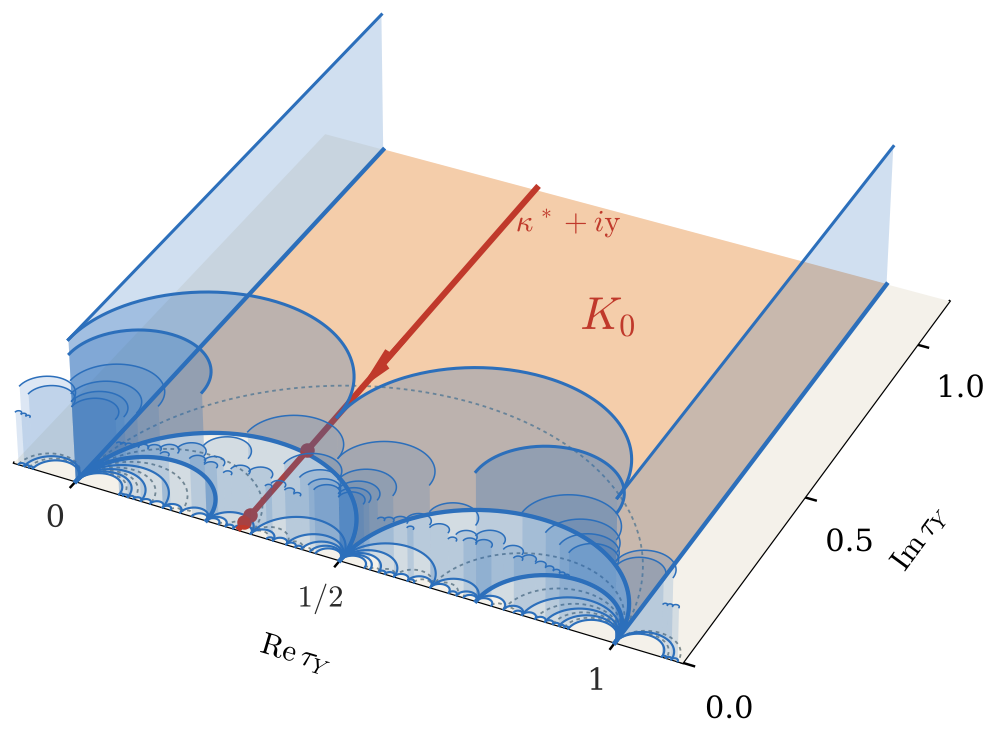
\includegraphics[width=0.8\textwidth]{fig_chambers.png}
\caption{Walls and chambers in the upper half-plane of $\tau_Y$. The walls are the Farey geodesics with an even denominator, drawn as curtains; the Farey geodesics with two odd denominators (dashed) are not walls. The shaded region is the chamber $K_0$, the ideal quadrilateral with vertices $0,\frac12,1,\infty$, in which the polar coefficients of $\varphi^F_m$ are read off. The path $\kappa^*+i\mathsf y$ of the proof of Theorem~\ref{thm:Pinf} descends from $K_0$ and crosses finitely many walls (dots), each contributing one term of the wall sum.}\label{fig:chambers}
\end{figure}

\subsection{Proof of Theorem~\ref{thm:Pinf}}
Fix a polar term $T=(m,\nu,\tilde\ell)$, and let $\omega_0$, $t$, $\delta$ be as in Section~\ref{sec:walls}; so $0\le\omega_0<1$ and $\delta>0$. Call a non-vertical wall $G$ \emph{relevant} if $m_G\ge-1$ and $n_G\ge-1$; by Corollary~\ref{cor:transport} and the definition of $d_1$, only relevant walls have a nonzero jump.

\begin{lemma}\label{lem:finite}
Let $0<\delta'<\delta$ and $J=[\omega_0-\delta',\omega_0+\delta']$. Every relevant wall whose open interval $(q/s,p/r)$ meets $J$ has $r,s\le(1/m+2\delta'+1)/(\delta^2-\delta'^2)$. In particular there are finitely many such walls.
\end{lemma}

\begin{proof}
Let $q/s<\kappa<p/r$ with $\kappa\in J$, put $U'=p/r-\kappa$, $W'=\kappa-q/s$, so $U',W'>0$, $U'+W'=1/rs$, and $h=\kappa-\omega_0$, $|h|\le\delta'$. By Lemma~\ref{lem:walls}(ii) (whose formulas for $m_G$, $n_G$ hold for every $G$), $m_G\ge-1$ means $(U'+h)^2\ge\delta^2-1/(mr^2)$. Since $|U'+h|\le1/(rs)+\delta'$ and $rs\ge r$, $r^2\ge r$,
\[
\delta^2-\delta'^2\le\frac{2\delta'}{rs}+\frac1{r^2s^2}+\frac1{mr^2}\le\frac{2\delta'+1+1/m}{r},
\]
which bounds $r$; $n_G\ge-1$ and $W'$ bound $s$ in the same way. For given $r,s$ the endpoint $p/r$ lies in $(\omega_0-\delta',\omega_0+\delta'+1)$, which leaves finitely many $p$, and $q$ is then determined by $ps-qr=1$.
\end{proof}

Let $\delta'=\delta/2$, let $\mathcal E$ be the finite set of endpoints greater than $\omega_0$ of the relevant walls of Lemma~\ref{lem:finite}, and let $\beta=\min(\mathcal E\cup\{\omega_0+\delta',1\})>\omega_0$. Choose $\kappa^*=(2j+1)/2^k\in(\omega_0,\beta)$ with $k$ so large that
\[
V(\kappa^*)=4^km\big((\kappa^*-\omega_0)^2-\delta^2\big)\le4^km(\delta'^2-\delta^2)\le-2 .
\]
Consider the path $\gamma(\mathsf y)=\kappa^*+i\mathsf y$, $\mathsf y$ decreasing from $+\infty$ to $0$ (Figure~\ref{fig:chambers}). For $\mathsf y>\frac14$ it lies in $K_0$, because $0<\kappa^*<1$. By Lemma~\ref{lem:farey}(F3), a Farey edge whose interval contains $\kappa^*$ strictly has denominators adding up to at most $2^k$, so $\gamma$ meets finitely many walls, each exactly once, transversally, passing from outside to inside; it meets no vertical wall. Distinct walls meet $\gamma$ at distinct heights by (F1). Between consecutive walls $\gamma$ stays in one chamber (it may cross odd edges), and below the last one it stays in the chamber $C$ of Lemma~\ref{lem:vanish}(ii) for $\kappa=\kappa^*$, where the coefficient of $T$ vanishes since $V(\kappa^*)\le-2$. Summing Corollary~\ref{cor:transport} along $\gamma$,
\[
d(T;K_0)=d(T;K_0)-d(T;C)=\sum_{G:\ q/s<\kappa^*<p/r}J_G(T).
\]
Only relevant walls contribute. A relevant wall with $q/s<\kappa^*<p/r$ meets $J$, so $p/r\in\mathcal E$ or $p/r\le\omega_0$; the latter is excluded by $p/r>\kappa^*>\omega_0$, so $p/r>\omega_0$, and $q/s\le\omega_0$ because otherwise $q/s\in\mathcal E$ and $q/s>\kappa^*$. Conversely, a relevant wall with $q/s\le\omega_0<p/r$ has an interval meeting $J$, so $p/r\in\mathcal E$, $p/r>\kappa^*$ and $q/s<\kappa^*$. Hence the sum runs over the relevant walls in $\mathcal W(m,\nu,\tilde\ell)$, and since $a_I(\nu,\tilde\ell)=\sum_{G\in\mathcal W(m,\nu,\tilde\ell)}J_G(T)$ by \eqref{eq:Pinf}, it equals $a_I(\nu,\tilde\ell)$; the remaining $G\in\mathcal W(m,\nu,\tilde\ell)$ (odd edges, or not relevant) contribute $0$. By Proposition~\ref{prop:identification}, $d(T;K_0)=c^F_m(2\nu,\tilde\ell)$. \qed

\begin{remark}\label{rem:convention}
The opposite endpoint convention, $q/s<\omega_0\le p/r$, gives the same value. If $\omega_0>0$, choose $\kappa^*$ slightly to the left of $\omega_0$, in $(0,\omega_0)$ and closer to $\omega_0$ than every endpoint smaller than $\omega_0$ of the walls of Lemma~\ref{lem:finite}; the argument above applies verbatim. If $\omega_0=0$, then $\tilde\ell=0$, the path starts in $K_0'$, and $d(T;K_0')=d(T;K_0)$ by Lemma~\ref{lem:jump}. In particular no averaging over the two conventions is needed when $2m\mid\tilde\ell$.
\end{remark}

\begin{remark}\label{rem:notused}
The proof does not use the global meromorphy of $1/\Phit_6$ on the Siegel upper half-space, the identification of $\Phit_6$ with a Borcherds lift or with the square of a theta-type form, nor \cite[Theorem~5.2]{BSS25}: the meromorphy of $\varphi_m$, its poles and the holomorphy of $\varphi^F_m$ are proved in Proposition~\ref{prop:identification} from the product formula. The formula \eqref{eq:polar} for the polar part is taken from \cite[(5.45)]{BSS25} as a definition.
\end{remark}
